\documentclass[11pt]{article}
\usepackage[utf8]{inputenc}
\usepackage{algorithm}
\usepackage{algorithmic}
\usepackage{amsfonts}
\usepackage{amsmath}
\usepackage{amssymb}
\usepackage{amsthm}
\usepackage[english]{babel}
\usepackage{booktabs}
\usepackage[labelfont=bf]{caption}
\usepackage{chngcntr}
\usepackage{color, colortbl}
\usepackage{fancyhdr}
\usepackage{graphicx}
\usepackage[utf8]{inputenc}
\usepackage[numbers]{natbib}
\usepackage{parskip}
\usepackage{subcaption}

\usepackage[vcentering,dvips]{geometry}
\geometry{
    papersize={7in,9in},
    bottom=3pc,
    top=5pc,
    left=5pc,
    right=5pc,
    bmargin=4.5pc,
    footskip=18pt,
    headsep=25pt}


\usepackage[
  colorlinks=true,
  linkcolor=black,
  anchorcolor=black,
  citecolor=black,
  filecolor=black,
  menucolor=black,
  runcolor=black,
  urlcolor=black]{hyperref}

\definecolor{Gray}{gray}{0.9}
\newcommand{\dotscale}{0.7}

\theoremstyle{definition}
\renewcommand\qedsymbol{$\blacksquare$}
\newtheorem{example}{Example}[section]

% Section numbers in captions.
\counterwithin{figure}{section}
\counterwithin{table}{section}
\counterwithin{example}{section}
\counterwithin{algorithm}{section}

\fancyhf{}
\lhead{\leftmark}
\rhead{\thepage}
\pagestyle{fancy}

%% log-sum-exp
\DeclareMathOperator*{\LSE}{\textrm{LSE}}

%% Matrices
\newcommand{\mA}{{\bf A}}
\newcommand{\mB}{{\bf B}}
\newcommand{\mC}{{\bf C}}

%% Vectors
\newcommand{\vr}{{\bf r}}
\newcommand{\vu}{{\bf u}}
\newcommand{\vv}{{\bf v}}

%% Graphs
\newcommand{\gA}{\mathcal{A}}
\newcommand{\gB}{\mathcal{B}}
\newcommand{\gC}{\mathcal{C}}
\newcommand{\gE}{\mathcal{E}}
\newcommand{\gT}{\mathcal{T}}
\newcommand{\gY}{\mathcal{Y}}
\newcommand{\gZ}{\mathcal{Z}}

%% <s> and </s> tokens
\newcommand{\sos}{\textrm{<s>}}
\newcommand{\eos}{\textrm{</s>}}


\title{An Introduction to Weighted Automata \\ in Machine Learning}
\author{Awni Hannun\footnote{
  Send correspondence to
  \href{mailto:awni.hannun@gmail.com}{awni.hannun@gmail.com}}}

\begin{document}

\maketitle

\begin{abstract}
    The goal of this work is to introduce the reader to weighted finite-state
    automata and their application to machine learning. I begin by motivating
    the use of automata in machine learning and proceed with an introduction to
    acceptors, transducers, and their associated properties. Many of the core
    operations of weighted automata are then described in detail. Following
    this, the work moves closer to the research frontier by explaining
    automatic differentiation and its use with weighted automata. The last
    section presents several extended examples to gain deeper familiarity with
    weighted automata, their operations, and applications to machine-learning.
\end{abstract}

\tableofcontents

\documentclass[main.tex]{subfiles}
\begin{document}

\section{Introduction}
\label{sec:introduction}

Relatively speaking, finite-state automata have a long history of application
in machine learning. The majority of these applications involve sequential
data.  For example, they are or have been used in speech recognition, machine
translation and other natural language tasks, and protein function analysis and
other tasks in computational biology.

However, the application of these data structures in machine learning is far
from main stream. In fact, their use likely decreased with the advent of
end-to-end deep learning. The recent development of frameworks for automatic
differentation with automata suggests there may be renewed interest in the
application of automata to machine learning.

This tutorial introduces weighted automata and their operations. Once this
fundamental data structure is well understood, we then continue to build our
intuition by working through some extended examples.  I hope at minimum this
tutorial engenders an appreciation for the potential of automata in machine
learning. Ideally for some readers this tutorial will be a launching point for
the incorporation of automata in machine-learning research and applications.

However, before launching into the more technical content, let's start with
some broader perspectives in order to motivate the use of automata in machine
learning.

\subsection{Monolothic or Modular}

In the past, complex machine-learning systems, like those used in speech
recognition, involved many specialised hand-endingeered components. The trend
is now for the opposite. Most machine-learning applications involve a single,
monolithic neural network. Both of these extremes have advantages and both have
disadvantages.

I believe a primary advantage of automata in machine learning is their
ability to harness the best of both worlds. Automata are capable of retaining
many if not all of the advantages of a multi-componenet, hand-engineered system
as well as those of a monolothic deep neural network. The next few paragraphs
explain some of these advantages and the regime to which they apply.

\paragraph{Modular:} One of the advantages of multi-component, hand-engineered
systems over monolothic neural networks is modularity. In traditional software
design modularity is usually a good thing. Modular systems are easier to
develop since part of the system can be changed without needing to change the
rest. In machine-learning systems, modularity is useful to avoid retraining the
entire system when only part of the model needs to be updated. Modularity can
also be useful when the individual modules can be reused. For example, speech
recognition systems are built from acoustic models and language models.
Acoustic models can be language agnostic and used for different languages.
Language models are general text based models which can be used in many
different tasks.

\paragraph{Compound errors:} A primary disadvantage of modular systems is that
errors compound. Each module is typically developed in isolation and hence
unaware of the types of errors made by the modules from which it receives
input. Monolothic systems on the other hand can be thought of as being
constructed from many sub-components all of which are jointly optimized towards
a single goal. These subcomponents can learn to compensate for the mistakes
made by the others and in general work together more seamlessly.

\paragraph{Adaptable:} Modular systems are typically more adaptable than
monolothic systems. A machine-learning model which is tuned for one domain
usually won't work in another domain without retraining at least part of the
model on data from the new domain. Monolothic neural networks typically require
a lot of data and hence are difficult to adapt to new domains. Modular systems
must also be adapted. However, in some cases only one or a small subset of the
modules need be updated, making the adaptation problem simpler.

\paragraph{Learns from data:} One of the hallmarks of deep neural networks is
their ability to continue to learn and improve with larger data sets. Because
of the many assumptions hard-wired into more traditional modular systems, they
hit a performance ceiling much earlier as data set sizes increase. Retaining
the ability to learn when data is plentiful is a critical features of any
machine-learning system.

\paragraph{Prior knowledge:} On the other hand, one of the downsides of deep
neural networks is their need for large data sets to yield even decent
performance. Encoding prior knowledge into a model improves sample efficiency
and hence reduces the need for data. Encoding prior knowledge into a deep
neural networks is not easy. In some cases, encoding prior knowledge into a
neural network can be done, such as the translation invariance of convolutions.
However, in general, this is not so straightforward. Modular systems by their
very nature incorporate prior knowledge for a give task. Each module is
designed and built to solve a specific sub-task, usually with plenty of
potential for customization towards that task.

Modular and monolothic systems have complementary advantages with respect to
these four traits. Ideally we could construct machine-learning models which
retain the best of each. Automata-based modeling is one possibility which will
task us a step closer towards this goal.  However, to use automata to their
full potential we have to overcome a couple of challenges. The key is enabling
the use of weighted automata in training the model itself. This requires 1)
efficient implementations 2) easy to use frameworks which support automatic
differentiation.

\subsection{Advantages of Differentiable Automata}

A key to unlocking the potential of automata in machine learning is enabling
their use during the training stage machine-learning models. All of the
operations I introduce later are differentiable with respect to the arc weights
of their input graphs. This means that weighted automata and the operations on
them can be used in a similar manner as tensors and their corresponding
operations are used in deep learning. Operations can be chained to form complex
computation graphs. Some of the weighted automata which are input to the
computation graph can have learnable parameters. These parameters can be
optimized using backpropagation and gradient descent.

Automatic differentiation makes computing gradients for complex computation
graphs much simpler. Hence combining automatic differentiation with weighted
automata is improtant to enabling their use in training machine-learning
models.

Sophisticated machine-learning systems often separate the training and
inference stages of the algorithm. Multiple models are trained in isolation via
one code path. For prediction on new data, the individual models are combined
and rely on a different code path. The constraints of the two regimes (training
and inference) are such that separation from a modeling and software
perspective is often the best option. However, this is not without drawbacks.

First, from a pragmatic standpoint, having separate logic and code paths for
training and inference requires extra effort and usually results in bugs from
subtle mismatches between the two paths. Second, from a modeling standpoint,
optimizing individual models in isolation and then combining them is often
sub-optimal.

One of the benefits of combining automatic differentiation with weighted
automata is the potential to bring the training and inference stages closer
together. For example, speech recognizers often use hand-implemented loss
functions at training time. However, the decoder (used for inference) brings
together mutliple models represented as graphs (lexicon, language model,
acoustic model, \emph{etc.}) in a completely different code path. By enabling
automatic differentiotion with graphs, the decoding stage can also be used for
training.  This has the potential to both simplify and improve the performance
of the system.

Loss functions like Connectionist Temporal Classification, the Automatic
Segmentation criterion, and Lattice-free Maximum Mutual Information are
implmeented with custom and highly optimized software. However, these loss
functions can all be implemented using graphs and (differentiable) operations
on graphs.

This separation of code from data, where graphs represent the data and
operations on graphs represent the code, has several benefits. First, the separation
simplifies the software. Second, the separation facilitates research by making
it easier to experiment with new ideas. Lastly, the separation enables the
optimization of graph operations to be more broadly shared.

\subsection{Comparison to Tensors}

Modern deep learning is built upon the tensor data structure and the many
operations which take as input one or more tensors. Some of the more common
operations include matrix multiplicatoin, 2-dimensional convolution, reduction
operations, and unary and binary operations.

Automata are an alternative data structure and the operations are quite
different in general. However, one can draw a loose analogy between the
operations on automata and those on tensors.
Table~\ref{tab:tensor_wfst_analogy} shows some of the common operations on
tensors and their analogous operations on automata. The analogy is quite loose,
but still useful at the very least as a mnemonic device and perhaps can help
build intuition for the various operations on graphs.

For example, superficially the formula for matrix multiplication and transducer
composition are quite similar. Assume we have three matrices such that $\mC = \mA
\mB$, then the $(i, j)$ element of $\mC$ is given by:
\begin{equation}
    C_{ij} = \sum_{k} A_{ik} B_{kj}
\end{equation}
Assume we have three transducers (graphs) where $\gC$ is the composition of
$\gA$ and $\gB$ , then the score of the path pair $(\vu, \vv)$ is given by:
\begin{equation}
    \mathcal{C}(\vu, \vv) = \LSE_{\vr} \mathcal{A}(\vu, \vr) + \mathcal{B}(\vr, \vv),
\end{equation}
where $\LSE$ is the \emph{log-sum-exp} operation (we will describe composition
in much more detail in section~\ref{sec:advanced_operations}). Both operations
take on the form of an accumulation over an inner variable of values from each
of the inputs. In matrix multiplication this is the shared dimnsion of the
matrices $\mA$ and $\mB$. In graph composition the inner variable is the shared
path $\vr$.

\begin{table}[ht]
    \renewcommand{\arraystretch}{1.4}
    \caption{The table shows loosely analogous operations between tensors and
    automata (acceptors and transducers).}
    \centering
    \begin{tabular}{l l l}
    \toprule
        Tensor & Automata \\
    \midrule
        Matrix multiplication, convolution & Intersect, compose \\
        \rowcolor{Gray} Reduction ops (sum, prod, \emph{etc.}) & Shortest distance (forward, Viterbi) \\
        Unary ops (power, negation, \emph{etc.})  & Unary ops (closure) \\
        \rowcolor{Gray} $n$-ary ops (addition, subtraction, \emph{etc.})  & $n$-aryops (concatenation, union) \\
    \bottomrule
    \end{tabular}
    \label{tab:tensor_wfst_analogy}
\end{table}

A higher-level analogy to tensor-based deep learning can also be made. Modern
machine-learning frameworks like PyTorch and TensorFlow (and their ancestors
like Torch and Theano) were critical to the success of tensor-based deep
learning. These frameworks include support for automatic differentiation. They
also provide easy to use access to extremely efficient implementations of the
core operations. In the same way, automata-based machine learning should
benefit from frameworks with these features. We are just beginning to see new
developments in frameworks for automata-based machine learning including
GTN\footnote{I am a primary author of the GTN framework which is open source at
\url{https://github.com/gtn-org/gtn}} and K2\footnote{The K2 framework is the
successor of Kaldi and is open source at \url{https://github.com/k2-fsa/k2}}.
Perhaps these will encourage the use of automata in machine learning.

\subsection{Bibliographic Notes}

%% On Transducers in ML
%% a lot of Mohri's work

%% On frameworks
%% PyTorch, TensorFlow, Theano and Torhc
%% Open FST

%% On differentiable transducers
%% graph transformer networks, GTN, K2

\end{document}

\section{Acceptors and Transducers}
\label{sec:acceptors_transducers}

\subsection{Automata}
\label{sec:automata}

The broad class of graphs we are going to look at are finite-state automata.
These include deterministic finite-state automata (DFAs) and non-deterministic
finite-state automata (NFAs). More specifically we will consider a
generalization of DFAs and NFAs called weighted finite-state acceptors (WFSAs).
That's a mouthful, so I will just call them \emph{acceptors}. We will also
consider a further generalization of an acceptor called a \emph{transducer}
(weighted finite-state transducers or WFSTs). Figure~\ref{fig:wfsa_classes}
shows the relation between these three graphs; transducers, acceptors, and
automata. Transducers are the most expressive in terms of their
representational power, followed by acceptors followed by unweighted automata.

\begin{figure}
    \centering
    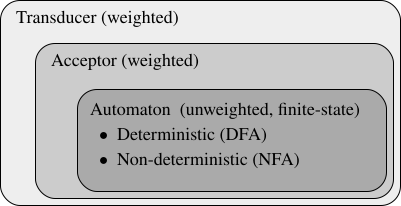
\includegraphics[width=0.7\linewidth]{figures/wfsa_classes}
    \caption{A hierarchy of automata classes from general to specific in terms
    of representation power. Weighted transducers can represent anything that
    weighted acceptors can represent. Weighted acceptors in turn can represent
    any unweighted finite-state automata.}
    \label{fig:wfsa_classes}
\end{figure}

Before we dive into acceptors and transducers, let's introduce some general
graph terminology that I will use throughout. In the following graph a
\emph{state} or \emph{node} is represented by a circle. The arrows represent
connections between two states. We usually refer to these as \emph{arcs} but
sometimes also \emph{edges}. The graph is directed since the connections
between states are unidirectional arrows. The arcs in a graph can have labels.
In figure~\ref{fig:simple_automata} the arc between states $0$ and $1$ has a
label of $a$. Similarly, the arc between states $1$ and $2$ has a label of $b$.
The graph is an example of a finite-state automata (FSA) or finite-state
machine (FSM), so called because it has a finite number of nodes.

\begin{figure}
    \centering
    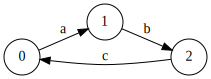
\includegraphics{figures/simple_automata}
    \caption{An example of a simple finite-state automata.}
    \label{fig:simple_automata}
 \end{figure}

An automata is deterministic if for each state and label pair there is only one
outgoing transition which matches that label. An automata is nondeterministic
if multiple transitions leaving a state have the same label. The graphs in
figure~\ref{fig:dfa_nfa} show an example of a deterministic and a
nondeterministic automata. In general, acceptors and transducers to can be
nondeterministic.

\begin{figure}
    \centering
    \begin{subfigure}[b]{0.48\textwidth}
        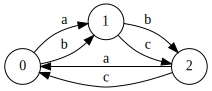
\includegraphics[scale=\dotscale]{figures/simple_dfa}
        \caption{Deterministic}
        \label{fig:simple_dfa}
    \end{subfigure}
    \begin{subfigure}[b]{0.48\textwidth}
        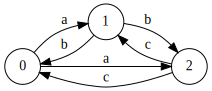
\includegraphics[scale=\dotscale]{figures/simple_nfa}
        \caption{Nondeterministic}
        \label{fig:simple_nfa}
    \end{subfigure}
    \caption{An example of a deterministic automata and a nondeterministic
    automata. The nondeterministic automata has two arcs leaving state $0$ both
    with label $a$ and two arcs leaving state $2$ both with the label $c$.}
    \label{fig:dfa_nfa}
\end{figure}

\subsection{Acceptors}

Let's start by constructing some very basic automata to get a feel for their
various properties.

The start state $s = 0$ has a bold circle around it. The accepting state $1$ is
represented with concentric circles. Each arc has a label and a corresponding
weight. So the first arc from state $0$ to state $1$ with the text $a/0$ means
the label is $a$ and the weight is $0$. The fact that there is only a single
label on each arc means this graph is an \emph{acceptor}. Since it has weights,
we say its a weighted acceptor. Since the number of states is finite, some
would call it a weighted finite-state acceptor or WFSA. Again, that's a
mouthful, so I'll just call these graphs acceptors.

\begin{figure}
    \centering
    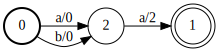
\includegraphics[scale=\dotscale]{figures/simple_fsa}
    \caption{An example of a simple acceptor. The label on each arc shows the
    input label and weight, so the $a/0$ represents a label of $a$ and a weight
    of $0$.}
    \label{fig:simple_fsa}
\end{figure}

An accepting path in the graph is a sequence of arcs which begin at a start
state and end in an accepting state. By concatenating the labels on an
accepting path, we get a string which is accepted by the graph. So the string
$aa$ is accepted by the graph by following the state sequence $0 \rightarrow 2
\rightarrow 1$. The string $ba$ is also accepted by the graph by following the
same state sequence but taking the arc with label $b$ when traversing from
state $0$ to state $1$. The language of the acceptor is the set of all strings
which are accepted by it. You may also encounter ``recognized'' used as a
synonym for ``accepted''. Let the variable $\gA$ represent the acceptor in
figure~\ref{fig:simple_fsa}. In general, I'll use uppercase script letters to
represent graphs. Let $\mathcal{L}(\gA)$ denote the language of $\gA$. In this
case $\mathcal{L}(\gA) = \{aa, ba\}$.

There are different ways to compute the weight of a string accepted by the
graph. The most common is to sum the weights of the arcs on the accepting path
for that string. For example the string $aa$ in the graph in
figure~\ref{fig:simple_fsa} has a weight of $0 + 2 = 2$. Another option would
be to multiply the weights. These two options correspond to interpreting the
weights as either log probabilities or probabilities. We'll have more to say
about this later.

The graph in figure~\ref{fig:multi_path} accepts the same sequence by multiple
paths.

\begin{figure}
    \centering
    \includegraphics[scale=\dotscale]{figures/multi_path}
    \caption{An acceptor which has multiple paths for the same sequence, $aa$.}
    \label{fig:multi_path}
\end{figure}

The string $aa$ is accepted along the state sequence $0 \rightarrow 2
\rightarrow 1$ and along the state sequence $0 \rightarrow 3 \rightarrow 1$. In
this case, to compute the score of $aa$ we need to consider both paths. Again
we have a couple of options here. The most common approach is to
\emph{log-sum-exp} the individual path scores. Again this corresponds to
interpreting the path scores as log probabilities. We'll use $\LSE(s_1, s_2)$
to denote the \emph{log-sum-exp} of the two scores $s_1$ and $s_2$:
\begin{equation}
\LSE(s_1, s_2) = \log \left( e^{s_1} + e^{s_2}\right).
\end{equation}
So the overall weight for the string $aa$ in the graph in
figure~\ref{fig:multi_path} is given by:
$$
\log \left(e^{0 + 2} + e^{1 + 3}\right) = 4.13.
$$

Acceptors can have multiple start states and multiple accept states. In the
graph in figure~\ref{fig:multi_start_accept}, the states $0$ and $1$ are both
start states, and the states $3$ and $4$ are both accept states.

\begin{figure}
    \centering
    \includegraphics[scale=\dotscale]{figures/multi_start_accept}
    \caption{An acceptor with multiple start states ($0$ and $1$) and multiple
    accept states ($3$ and $4$).}
    \label{fig:multi_start_accept}
\end{figure}

It turns out that allowing multiple start or accept states does not increase
the expressive power of the graph. With $\epsilon$ transitions (which we will
discuss soon), one can convert any graph with multiple start states and
multiple accept states into an equivalent graph with a single start state and a
single accept state.

Note also that start states can have incoming arcs (as in state $1$) and accept
states can have outgoing arcs, as in state $3$.

\begin{example}
Compute the score of the string $ab$ in figure~\ref{fig:multi_start_accept}.
\end{example}

\begin{proof}[\unskip\nopunct]
The two state sequences which accept the string $ab$ are the states $0
\rightarrow 2 \rightarrow 3$ and $1 \rightarrow 3 \rightarrow 4$. The overall
score is given by:
$$
\log (e^{1 + 3} + e^{1 + 2}) = 4.31.
$$
\end{proof}

Graphs can also have self-loops and cycles. For example, the graph in
figure~\ref{fig:fsa_loops} has a self-loop on the state $0$ and a cycle
following the state sequence $0 \rightarrow 1 \rightarrow 2 \rightarrow 0$.

\begin{figure}
    \centering
    \includegraphics[scale=\dotscale]{figures/fsa_loops}
    \caption{A graph with a self-loop on the state $0$ and a cycle from $0
    \rightarrow 1 \rightarrow 2 \rightarrow 0$.}
    \label{fig:fsa_loops}
\end{figure}

The language of a graph with cycles and self-loops contains infinitely many
strings.  For example, the language of the graph in figure~\ref{fig:fsa_loops}
includes any string that starts with zero or more $a$s and ends in $bb$. As a
regular expression we write this as $a^*bb$ where the $^*$ denotes zero or more
$a$s.

The $\epsilon$ symbols has a special meaning when it is the label on an arc.
Any arc with an $\epsilon$ label can be traversed without consuming an input
token in the string. So the graph in figure~\ref{fig:fsa_epsilon} accepts the
string $ab$, but it also accepts the string $b$ because we can traverse from
state $0$ to state $1$ without consuming an input.

\begin{figure}
    \centering
    \includegraphics[scale=\dotscale]{figures/fsa_epsilon}
    \caption{An acceptor with an $\epsilon$ transition on the second arc
    between state $0$ and $1$.}
    \label{fig:fsa_epsilon}
\end{figure}

As it turns out, any graph with $\epsilon$-transitions can be converted to an
equivalent graph without $\epsilon$ transitions. However, this usually comes at
a large cost in the size of the graph. Complex languages can be represented by
much more compact graphs with the use of $\epsilon$-transitions.

\begin{example}
Convert the graph in figure~\ref{fig:multi_start_accept} which has multiple
start and accept states to an equivalent graph with only a single start and
accept state using $\epsilon$ transitions.
\end{example}

\begin{proof}[\unskip\nopunct]
The graph in figure~\ref{fig:epsilon_start_accept} is the equivalent graph
with a single start state and a single accept state.

\begin{figure}
    \centering
    \includegraphics[scale=\dotscale]{figures/epsilon_start_accept}
    \caption{The equivalent graph using only a single start state and accept
    state to the graph in figure~\ref{fig:multi_start_accept} which has
    multiple start and accept states.}
    \label{fig:epsilon_start_accept}
\end{figure}

The construction works by creating a new start state and connecting it to the
old start states with $\epsilon$ transitions with a weight of $0$. The old
start nodes are regular internal nodes in this new graph. Similarly the old
accept states are now regular states and they connect to the new accept state
with $\epsilon$ transitions with a weight of $0$.
\end{proof}

\subsection{Transducers}

A \emph{transducer} maps input strings to output strings. Transducers are a
generalization of acceptors. Every acceptor is a transducer, but not every
transducer is an acceptor. Let's look at a few example transducers to
understand how they work.

The arc labels distinguish an acceptor from a transducer. A transducer has both
an input and output arc label. The arc labels are of the form $a\!:\!x/0$ where
$a$ is the input label $x$ is the output label and $0$ is the weight. An
acceptor can be represented as a transducer where the input and output labels
on every arc are identical.

\begin{figure}
    \centering
    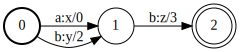
\includegraphics[scale=\dotscale]{figures/simple_fst}
    \caption{An example of a simple transducer. The label on each arc shows the
    input label, the output label, and the weight. So $a\!:\!x/0$ represents an
    input label of $a$, and output label of $x$, and a weight of $0$.}
    \label{fig:simple_fst}
\end{figure}

Instead of saying that a transducer accepts a given string, we say that it
\emph{transduces} one string to another. The graph in
figure~\ref{fig:simple_fst} transduces the string $ab$ to the string $xz$ and
the string $bb$ to the string $yz$. The weight of a transduced pair is
computed in the same way as in an acceptor. The scores of the individual arcs
on the path are summed. The path scores are combined with \emph{log-sum-exp}.
So the weight of the transduced pair $(ab, xz)$ in the graph in
figure~\ref{fig:simple_fst} is $0+3 = 3$.

We have to generalize concept of the language from an acceptor to a transducer.
I'll call this generalization the transduced set. Since it will always be clear
from context if the graph is an acceptor or transducer, I'll use the same
symbol $\mathcal{L}$ to represent the transduced set. If $\gT$ is a transducer,
then $\mathcal{L}(\gT)$ is the set of pairs of strings transduced by $\gT$.
More formally, a pair of strings $(\vx, \vy) \in \mathcal{L}(\gT)$ if $\gT$
transduces $\vx$ to $\vy$.

\begin{example}
Compute the score of the transduced pair $(aab, zyy)$ in the graph in
figure~\ref{fig:fst_example_score}.
\end{example}

\begin{proof}[\unskip\nopunct]
\begin{figure}
    \centering
    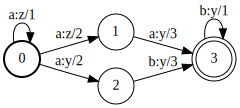
\includegraphics[scale=\dotscale]{figures/fst_example_score}
    \caption{An example transducer in which the sequence $aab$ is transduced to
    the sequence $zyy$ on multiple paths.}
    \label{fig:fst_example_score}
\end{figure}

The two paths which transduce $aab$ to $zyy$ are following the state sequence
$0 \rightarrow 1 \rightarrow 3 \rightarrow 3$ and $0 \rightarrow 0 \rightarrow
2 \rightarrow 3$. The score of the first path is $6$ and the score of the
second path is $6$. So the overall score is:
$$
\log \left(e^6 + e^6\right) = 6.69.
$$
\end{proof}

Transducers can also have $\epsilon$ transitions. The $\epsilon$ can be either
the input label on an arc, the output label on an arc, or both. When the
$\epsilon$ is the input label on an arc, it means we can traverse that arc
without consuming an input token, but we still output the arc's corresponding
output label. When the $\epsilon$ is the output label, the opposite is true.
The input is consumed but no output is produced. And when the $\epsilon$ is
both the input and the output label, the arc can be traversed without consuming
an input or producing an output.

\begin{figure}
    \centering
    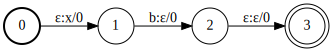
\includegraphics[scale=\dotscale]{figures/fst_epsilon}
    \caption{A transducer with $\epsilon$ transitions. The $\epsilon$ can be
    just the input label, just the output label, or both the input and output
    label.}
    \label{fig:fst_epsilon}
\end{figure}

In the graph in figure~\ref{fig:fst_epsilon}, the string $b$ gets transduced to
the string $x$. On the first arc between states $0$ and $1$, we output an $x$
without consuming any token. On the second arc between states $1$ and $2$, a
$b$ is consumed without outputting any new token. Finally, on the arc between
states $2$ and $3$ we neither consume nor output a token.

\section{Basic Operations}
\label{sec:basic_operations}

An operation on a transducer (or acceptor) takes one or more transducers as
input and outputs a transducer. You can think of these operations as functions
on graphs. As a reminder, I'll use uppercase script letters to represent
graphs, so $\gA$ for example can represent a graph. Functions will be denoted
by lower case variables. So $f(\gA)$ is a function which takes as input a
single graph and outputs a graph.

\subsection{Closure}

The closure, sometimes called the Kleene star, is a unary function (takes a
single input) which can operate on either an acceptor or transducer. If the
sequence $\vx$ is accepted by $\gA$, then zero or more copies of $\vx$ are
accepted by the closure of $\gA$. More formally, if the language of an acceptor
is $\L(\gA)$, then the language of the closure of $\gA$ is $\{\vx^n
\mid \vx \in \L(\gA),\;\; n = 0, 1, \ldots, \}$. The notation $\vx^n$
means $\vx$ concatenated $n$ times. So $\vx^2$ is $\vx \vx$ and $\vx^0$ is the
empty string. Usually the closure of an acceptor is denoted by $^*$, as in
$\gA^*$. This is the same notation used in regular expressions.

The closure of a graph is easy to construct with the use of $\epsilon$
transitions. The language of the graph in figure~\ref{fig:fsa_pre_closure} is
the string $aba$.

\begin{figure}
    \centering
    \includegraphics[scale=\dotscale]{figures/fsa_pre_closure}
    \caption{An example of a simple acceptor with language $\{aba\}$, in other
    words $\L(\gA) = \{aba\}$.}
    \label{fig:fsa_pre_closure}
\end{figure}

The closure of the graph needs to accept an arbitrary number of copies of $aba$
including the empty string. To accept the empty string we make the start state
an accept state as well. To accept one or more copies of $aba$ we simply wire
up the old accept states to the new start state with $\epsilon$ transitions.

The closure of the graph in figure~\ref{fig:fsa_pre_closure} is shown in
figure~\ref{fig:fsa_closure}.

\begin{figure}
    \centering
    \includegraphics[scale=\dotscale]{figures/fsa_closure}
    \caption{The closure $\gA^*$ of the graph in
    figure~\ref{fig:fsa_pre_closure}. The language of the graph is $\{\epsilon,
    aba, abaaba, \ldots\}$.}
    \label{fig:fsa_closure}
\end{figure}

\begin{example}
You might notice that state $4$ in the graph in figure~\ref{fig:fsa_closure} is
not necessary. Consider an alternate construction for computing the
closure of a graph. We could have made the state $0$ into an accept state
and connected state $3$ to state $0$ with an $\epsilon$ transition, as in
the graph in figure~\ref{fig:fsa_closure_2}.

\begin{figure}
    \centering
    \includegraphics[scale=\dotscale]{figures/fsa_closure_2}
    \caption{The closure $\gA^*$ of the graph in
    figure~\ref{fig:fsa_pre_closure} using an alternate, simpler construction
    which connects the accept state to the original start state with an
    $\epsilon$ transition. This construction does not work for every case.}
    \label{fig:fsa_closure_2}
\end{figure}

For the graph in figure~\ref{fig:fsa_pre_closure}, this alternate construction
works and requires fewer states and arcs. In the general case, this
construction turns every start state into an accept state instead of adding
a new start state. Give an example where this doesn't work? In other words,
give an example where the graph from this modified construction is not the
correct closure of the original graph.
\end{example}

\begin{proof}[\unskip\nopunct]
An example for which the alternate construction does not work is shown in the
graph in figure~\ref{fig:fsa_pre_closure_wrong}. The language of the graph
is $a^nb$ (any number of $a$'s followed by a $b$) and the closure is
$(a^nb)^*$, or any sequence that ends with $b$.

\begin{figure}
    \centering
    \includegraphics[scale=\dotscale]{figures/fsa_pre_closure_wrong}
    \caption{An acceptor for which the alternate construction for the closure
    does not yield the correct result.}
    \label{fig:fsa_pre_closure_wrong}
\end{figure}

If we follow the modified construction for the closure, as in the graph in
figure~\ref{fig:fsa_closure_wrong}, then the language would incorrectly
include sequences that do not end with $b$ such as $a^*$. The graph
following the correct construction of the closure is in
figure~\ref{fig:fsa_closure_right}.

\begin{figure}
    \centering
    \includegraphics[scale=\dotscale]{figures/fsa_closure_wrong}
    \caption{The alternate construction which incorrectly computes the closure
    of the graph in figure~\ref{fig:fsa_pre_closure_wrong}.}
    \label{fig:fsa_closure_wrong}
\end{figure}


\begin{figure}
    \centering
    \includegraphics[scale=\dotscale]{figures/fsa_closure_right}
    \caption{The correct closure of the graph in
    figure~\ref{fig:fsa_pre_closure_wrong} which has the language $(a^nb)^*$, which
    is any sequence which ends with $b$.}
    \label{fig:fsa_closure_right}
\end{figure}

\end{proof}

\subsection{Union}

The union takes as input two or more graphs and produces a new graph. The
language of the resultant graph is the union of the languages of the input
graphs. More formally let $\gA_1, \ldots, \gA_n$ be $n$ graphs. The language of
the union graph is given by $\{ x \mid x \in \gA_i \textrm{ for some } i = 1,
\ldots, n \}$. I'll occasionally use the $+$ sign to denote the union, as in
$\gU = \gA_1 + \gA_2$.

Since we let a graph have multiple start states and multiple accept states, the
union is  easy to construct. A state in the union graph is a start state if it
was a start state in one of the original graphs. A state in the union graph is
an accept state if it was an accept state in one of the original graphs.

Consider the three graphs in figure~\ref{fig:union_inputs} with languages
$\{ab, aba, abaa, \ldots\}$, $\{ba\}$, and $\{ac\}$ respectively.

\begin{figure}
    \centering
    \begin{subfigure}[b]{0.8\textwidth}
        \centering
        \includegraphics[scale=\dotscale]{figures/union_1}
        \caption{}
    \end{subfigure}
    \par\bigskip
    \begin{subfigure}[b]{0.8\textwidth}
        \centering
        \includegraphics[scale=\dotscale]{figures/union_2}
        \caption{}
    \end{subfigure}
    \par\bigskip
    \begin{subfigure}[b]{0.8\textwidth}
        \centering
        \includegraphics[scale=\dotscale]{figures/union_3}
        \caption{}
    \end{subfigure}
    \caption{Three acceptors with languages $\{ab, aba, abaa, \ldots\}$,
    $\{ba\}$, and $\{ac\}$ from left to right, respectively.}
    \label{fig:union_inputs}
\end{figure}

Notice in the union graph in figure~\ref{fig:union} the only visual distinction
from the individual graphs is that the states are numbered consecutively from
$0$ to $8$ indicating a single graph with nine states instead of three
individual graphs. The language of the union graph is $\{ab, aba, abaa,
\ldots\} \cup \{ba\} \cup \{ac\}$.

\begin{figure}
    \centering
    \includegraphics[scale=\dotscale]{figures/union}
    \caption{The union of the three acceptors in figure~\ref{fig:union_inputs}
    with language $\{ab, aba, abaa, \ldots\} \cup \{ba\} \cup \{ac\}$.}
    \label{fig:union}
\end{figure}

\subsection{Concatenation}

Like union, concatenation produces a new graph given two or more graphs as
input. The language of the concatenated graph is the set of strings which can
be formed by any concatenation of strings from the individual graph.
Concatenation is not commutative, the order of the input graphs matters. More
formally the language of the concatenated graph is given by $\{\vx_1 \ldots
\vx_n \mid \vx_1 \in \L(\gA_1), \ldots, \vx_n \in \L(\gA_n)\}$. Occasionally, I
will denote concatenation by placing the graphs side-by-side. So $\gA_1 \gA_2$
represents the concatenation of $\gA_1$ and $\gA_2$.

The concatenated graph can be constructed from the original input graphs by
connecting the accept states of one graph to the start states of the next.
Assume we are concatenating $\gA_1, \ldots, \gA_n$. The start states of the
concatenated graph are the start states of the first graph, $\gA_1$. The accept
states of the concatenated graph are the accept states of the last graph,
$\gA_n$. For any two graph $\gA_i$ and $\gA_{i+1}$, we connect each accept
state of $\gA_i$ to each start state of $\gA_{i+1}$ with an $\epsilon$
transition.

\begin{figure}
    \centering
    \begin{subfigure}[b]{0.48\textwidth}
        \centering
        \includegraphics[scale=\dotscale]{figures/concat_1}
    \end{subfigure}
    \begin{subfigure}[b]{0.48\textwidth}
        \centering
        \includegraphics[scale=\dotscale]{figures/concat_2}
    \end{subfigure}
    \caption{The acceptor on left has language $\{ba\}$ and the acceptor on the
    right has language $\{ac, bc\}$.}
    \label{fig:concat_inputs}
\end{figure}

As an example, consider the two graphs in figure~\ref{fig:concat_inputs}. The
concatenated graph is in figure~\ref{fig:concat} and has the language $\{baac,
babc\}$.

\begin{figure}
    \centering
    \includegraphics[scale=\dotscale]{figures/concat}
    \caption{The graph is the concatenation of the two graphs in
    figure~\ref{fig:concat_inputs} and has the language $\{baac, babc\}$.}
    \label{fig:concat}
\end{figure}

\begin{example}
What is the identity graph for the concatenation function? The identity in a
binary operation is the value which when used in the operation leaves the second
input unchanged. In multiplication this would be $1$ since $c * 1 = c$ for any
real value $c$.

What is the equivalent of the annihilator graph in the concatenation function?
The annihilator in a binary operation is the value such that the operation with
the annihilator always returns the annihilator. For multiplication $0$ is the
annihilator since $c *0 = 0$ for any real value $c$.
\end{example}

\begin{proof}[\unskip\nopunct]
The graph which accepts the empty string is the identity. The graph which does
not accept any strings is the annihilator. See the
figure~\ref{fig:concat_identity_annihilator} for an example of these two
graphs.

\begin{figure}
    \centering
    \begin{subfigure}[b]{0.48\textwidth}
        \centering
        \includegraphics[scale=\dotscale]{figures/concat_identity}
        \caption{Identity}
        \label{fig:concat_identity}
    \end{subfigure}
    \begin{subfigure}[b]{0.48\textwidth}
        \centering
        \includegraphics[scale=\dotscale]{figures/concat_annihilator}
        \caption{Annihilator}
        \label{fig:concat_annihilator}
    \end{subfigure}
    \caption{The identity and the annihilator for the concatenation operation.
    The language of the identity graph is the empty string $\{\epsilon\}$. The
    language of the annihilator graph is the empty set $\{\}$.}
    \label{fig:concat_identity_annihilator}
\end{figure}

The identity graph is a single node which is both a start and accept state. The
language of the identity graph is the empty string. The annihilator graph is a
single non accepting state. The language of the annihilator graph is the empty
set. Note the subtle distinction between the language that contains the empty
string and the language that is the empty set. The former can be written as
$\{\epsilon\}$ whereas the latter is $\{\}$ (also commonly denoted by
$\varnothing$).
\end{proof}

\begin{example}
Construct the concatenation of the two graphs in
figure~\ref{fig:concat_example_inputs}.
\end{example}

\begin{proof}[\unskip\nopunct]

\begin{figure}
    \centering
    \begin{subfigure}[b]{0.48\textwidth}
        \centering
        \includegraphics[scale=\dotscale]{figures/concat_example_1}
    \end{subfigure}
    \begin{subfigure}[b]{0.48\textwidth}
        \centering
        \includegraphics[scale=\dotscale]{figures/concat_example_2}
    \end{subfigure}
    \caption{The acceptor on the right has the language $\{ba, bc\}$, the
    acceptor on the left has the language $\{a, c\}$.}
    \label{fig:concat_example_inputs}
\end{figure}

The concatenated graph is in figure~\ref{fig:concat_example}.

\begin{figure}
    \centering
    \includegraphics[scale=\dotscale]{figures/concat_example}
    \caption{The concatenation of the two graphs in
    figure~\ref{fig:concat_example_inputs} has the language $\{baa, bac, bca,
    bcc\}$.}
    \label{fig:concat_example}
\end{figure}

\end{proof}

\begin{example}
Suppose we have a list of graphs to concatenate $\gA_1, \ldots, \gA_n$ where the
$i$-th graph has $s_i$ start states and $a_i$ accept states. How many new
arcs will the concatenated graph require?
\end{example}

\begin{proof}[\unskip\nopunct]
For each consecutive pair of graphs $\gA_i$ and $\gA_{i+1}$, we need to add
$a_i * s_{i+1}$ connecting arcs in the concatenated graph. So the total
number of additional arcs is:
$$
\sum_{i=1}^{n-1} a_i * s_{i+1}.
$$
\end{proof}

\subsection{Summary}

We've seen three basic operations so far:

\begin{itemize}
    \item {\bf Closure:} The closed graph accepts any string in the input graph
        repeated zero or more times. The closure of a graph $\gA$ is denoted
        $\gA^*$.

    \item {\bf Union:} The union graph accepts any string from any of the input
        graphs. The union of two graphs $\gA_1$ and $\gA_2$ is denoted $\gA_1 +
        \gA_2$.

    \item {\bf Concatenation:} The concatenated graph accepts any string which
        can be formed by concatenating strings (respecting order) from the
        input graphs. The concatenation of two graphs $\gA_1$ and $\gA_2$ is
        denoted $\gA_1\gA_2$.

\end{itemize}

\begin{example}
Assume you are given the following individual graphs $\gA_a$, $\gA_b$, and
$\gA_c$, which recognize $a$, $b$, and $c$ respectively, as in
figure~\ref{fig:fsa_tokens}. Using only the closure, union, and
concatenation operations, construct the graph which recognizes any number
of repeats of the strings $aa$, $bb$, and $cc$. For example $aabb$ and
$bbaacc$ are in the language but $b$ and $ccaab$ are not.
\end{example}

\begin{proof}[\unskip\nopunct]

\begin{figure}
    \centering
    \begin{subfigure}[b]{0.32\textwidth}
        \centering
        \includegraphics[scale=\dotscale]{figures/fsa_a}
    \end{subfigure}
    \begin{subfigure}[b]{0.32\textwidth}
        \centering
        \includegraphics[scale=\dotscale]{figures/fsa_b}
    \end{subfigure}
    \begin{subfigure}[b]{0.32\textwidth}
        \centering
        \includegraphics[scale=\dotscale]{figures/fsa_c}
    \end{subfigure}
    \caption{The three individual automata with languages $\{a\}$, $\{b\}$, and
    $\{c\}$ from left to right, respectively.}
    \label{fig:fsa_tokens}
\end{figure}

First concatenate the individual graphs with themselves to get graphs which
recognize $aa$, $bb$, and $cc$. Then take the union of the three
concatenated graphs followed by the closure. The resulting graph is shown
in figure~\ref{fig:fsa_repeats}. The equation to compute the desired graph
is $\gA = (\gA_a\gA_a + \gA_b\gA_b + \gA_c\gA_c)^*$.

\begin{figure}
    \centering
    \includegraphics[scale=\dotscale]{figures/fsa_repeats}
    \caption{The even numbered repeats graph constructed from the individual
    token graphs using the operations $\gA = (\gA_a\gA_a + \gA_b\gA_b +
    \gA_c\gA_c)^*$.}
    \label{fig:fsa_repeats}
\end{figure}

\end{proof}

\documentclass[main.tex]{subfiles}

\begin{document}

\section{Advanced Operations}
\label{sec:advanced_operations}

\subsection{Intersect}

The intersection of two acceptors is the set of strings which is accepted by
both of them. The score of a path in the intersected graph is the sum of the
score of the path in each of the input graphs. More formally the language of
the intersected graph is given by $\{ \vx \mid \vx \in \L(\gA_1) \;\land\; \vx
\in \L(\gA_2)\}$.

The analagous operation for transducers is the composition, which we will
discuss in more detail in the next section. In most machine learning
applications, intersect and compose tend to be the primary operations used to
compute more complex graphs from simpler input graphs. Thus gaining a deeper
understanding of these two operations is worth the time.

We'll use the two graphs in figure~\ref{fig:intersect_inputs} to illustrate a
general algorithm for computing the intersection. In this case, the intersected
graph is easy to see by inspecting the two graphs. The only string which is
recognized by both graphs is the string $ab$, hence the intersected graph is
the graph which recognizes $ab$.

\begin{figure}
    \centering
    \begin{subfigure}[b]{0.48\textwidth}
        \centering
        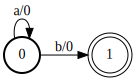
\includegraphics[scale=\dotscale]{figures/intersect_1}
    \end{subfigure}
    \begin{subfigure}[b]{0.48\textwidth}
        \centering
        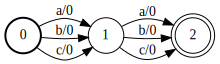
\includegraphics[scale=\dotscale]{figures/intersect_2}
    \end{subfigure}
    \caption{The acceptor on the left has a language of $a^*b$ and the acceptor
    on the right accepts all nine sequences of lenght $2$. The only sequence
    accepted by both, and hence is in the intersection, is the string $ab$.}
    \label{fig:intersect_inputs}
\end{figure}

The general algortihm relies on a queue to explore pairs of states from the two
input graphs. Pseudocode is given in algorithm~\ref{alg:intersect}.

\begin{algorithm}[t]
\caption{Intersect}
\label{alg:intersect}
\begin{algorithmic}[1]
\STATE \textbf{Input}: Acceptors $\gA_1$ and $\gA_2$
\STATE Initialize the queue $Q$ and the intersected graph $\gI$.

\FOR {$s_1$ and $s_2$ in all start state pairs of $\gA_1$ and $\gA_2$}
    \STATE Add $(s_1, s_2)$ to $Q$ and as a start state in $\gI$.
    \IF {$s_1$ and $s_2$ are accept states}
        \STATE Make $(s_1, s_2)$ an accept state in $\gI$.
    \ENDIF
\ENDFOR

\WHILE {$Q$ is not empty}
    \STATE Remove the next state pair $(u_1, u_2)$ from $Q$.
    \FOR {all arcs pairs $a_1$ and $a_2$ leaving $u_1$ and $u_2$ with matching labels}
        \STATE Get destination states $v_1$ of $a_1$ and $v_2$ of $a_2$.
        \IF {not yet seen $(v_1, v_2)$}
            \STATE Add $(v_1, v_2)$ as a state to $\gI$ and to $Q$.
            \IF {$v_1$ and $v_2$ are accept states}
                \STATE Make $(v_1, v_2)$ an accept state in $\gI$.
            \ENDIF
        \ENDIF
        \STATE Get the label $\ell$ of $a_1$.
        \STATE Get the weights $w_1$ of $a_1$ and $w_2$ of $a_2$.
        \STATE Add an arc from $(u_1, u_2)$ to $(v_1, v_2)$ with label $\ell$
        and weight $w_1 + w_2$.

    \ENDFOR
\ENDWHILE
\STATE \textbf{Return}: The intersected graph $\gI$.
\end{algorithmic}
\end{algorithm}


Some of the steps of the intersect algorithm on the two input graphs in
figure~\ref{fig:intersect_inputs} are shown in the sequence of graphs in
figure~\ref{fig:intersect_steps}. The states explored at each step are
highlighted in red. The intersected graph is the third graph on the right which
is constructed over the steps of the algorithm.

\begin{figure}
    \begin{subfigure}{\linewidth}
        \begin{minipage}{0.22\textwidth}
            \centering
            \includegraphics[scale=\dotscale]{figures/intersect_step_1_g1}
        \end{minipage}
        \begin{minipage}{0.37\textwidth}
            \centering
            \includegraphics[scale=\dotscale]{figures/intersect_step_1_g2}
        \end{minipage}
        \begin{minipage}{0.37\textwidth}
            \centering
            \includegraphics[scale=\dotscale]{figures/intersect_step_1_g_out}
        \end{minipage}
        \caption{The starts states in the input graphs are $0$ and $0$. So we
        add the start state $(0, 0)$ to the intersected graph and to the queue
        to be explored.}
    \end{subfigure}

    \begin{subfigure}{\linewidth}
        \begin{minipage}{0.22\textwidth}
            \centering
            \includegraphics[scale=\dotscale]{figures/intersect_step_2_g1}
        \end{minipage}
        \begin{minipage}{0.37\textwidth}
            \centering
            \includegraphics[scale=\dotscale]{figures/intersect_step_2_g2}
        \end{minipage}
        \begin{minipage}{0.37\textwidth}
            \centering
            \includegraphics[scale=\dotscale]{figures/intersect_step_2_g_out}
        \end{minipage}
        \caption{The first pair of outgoing arcs match on the label $a$. This
        means the downstream state $(0, 1)$ is reachable in the intersected
        graph. So we add $(0, 1)$ to the intersected graph and to the queue to
        be explored.}
    \end{subfigure}

    \begin{subfigure}{\linewidth}
        \begin{minipage}{0.22\textwidth}
            \centering
            \includegraphics[scale=\dotscale]{figures/intersect_step_3_g1}
        \end{minipage}
        \begin{minipage}{0.37\textwidth}
            \centering
            \includegraphics[scale=\dotscale]{figures/intersect_step_3_g2}
        \end{minipage}
        \begin{minipage}{0.37\textwidth}
            \centering
            \includegraphics[scale=\dotscale]{figures/intersect_step_3_g_out}
        \end{minipage}
        \caption{The next matching pair of outgoing arcs match on the label
        $b$. Also, we haven't visited the downstream state $(1, 1)$ yet. So we
        add $(1, 1)$ to the intersected graph and to the queue to be explored.}
    \end{subfigure}

    \begin{subfigure}{\linewidth}
        \begin{minipage}{0.22\textwidth}
            \centering
            \includegraphics[scale=\dotscale]{figures/intersect_step_4_g1}
        \end{minipage}
        \begin{minipage}{0.37\textwidth}
            \centering
            \includegraphics[scale=\dotscale]{figures/intersect_step_4_g2}
        \end{minipage}
        \begin{minipage}{0.37\textwidth}
            \centering
            \includegraphics[scale=\dotscale]{figures/intersect_step_4_g_out}
        \end{minipage}
        \caption{The arc in the second input graph with label $c$ does not have
        a matching arc from state $0$ in the first input graph, so it is
        ignored.}
    \end{subfigure}

    \begin{subfigure}{\linewidth}
        \begin{minipage}{0.22\textwidth}
            \centering
            \includegraphics[scale=\dotscale]{figures/intersect_step_5_g1}
        \end{minipage}
        \begin{minipage}{0.37\textwidth}
            \centering
            \includegraphics[scale=\dotscale]{figures/intersect_step_5_g2}
        \end{minipage}
        \begin{minipage}{0.37\textwidth}
            \centering
            \includegraphics[scale=\dotscale]{figures/intersect_step_5_g_out}
        \end{minipage}
        \caption{At this point we have considered all the matching outgoing
        arcs from $(0, 0)$ so we now move on to the next state pair in the
        queue, $(0, 1)$. From $(0, 1)$, a pair of outgoing arcs match on the
        label $a$. The downstream state $(0, 2)$ is new so we add it to the
        intersected graph and to the queue.}
    \end{subfigure}

\end{figure}

\begin{figure}\ContinuedFloat
    \begin{subfigure}{\linewidth}
        \begin{minipage}{0.22\textwidth}
            \centering
            \includegraphics[scale=\dotscale]{figures/intersect_step_6_g1}
        \end{minipage}
        \begin{minipage}{0.37\textwidth}
            \centering
            \includegraphics[scale=\dotscale]{figures/intersect_step_6_g2}
        \end{minipage}
        \begin{minipage}{0.37\textwidth}
            \centering
            \includegraphics[scale=\dotscale]{figures/intersect_step_6_g_out}
        \end{minipage}
        \caption{The next pair of matching outgoing arcs match on the label $b$
        and lead to the state pair $(1, 2)$. We add $(1, 2)$ to the queue and
        to the interescted graph. Also, since $1$ is an accept state in the
        first graph and $2$ is an accept state in the second graph, $(1, 2)$ is
        an accept state in the intersected graph.}
    \end{subfigure}

    \begin{subfigure}{\linewidth}
        \begin{minipage}{0.22\textwidth}
            \centering
            \includegraphics[scale=\dotscale]{figures/intersect_step_7_g1}
        \end{minipage}
        \begin{minipage}{0.37\textwidth}
            \centering
            \includegraphics[scale=\dotscale]{figures/intersect_step_7_g2}
        \end{minipage}
        \begin{minipage}{0.37\textwidth}
            \centering
            \includegraphics[scale=\dotscale]{figures/intersect_step_7_g_out}
        \end{minipage}
        \caption{Again, the arc in the second input graph with label $c$ does
        not have a matching arc from state $0$ in the first input graph, so it
        is ignored.}
    \end{subfigure}

    \begin{subfigure}{\linewidth}
        \begin{minipage}{0.22\textwidth}
            \centering
            \includegraphics[scale=\dotscale]{figures/intersect_step_8_g1}
        \end{minipage}
        \begin{minipage}{0.37\textwidth}
            \centering
            \includegraphics[scale=\dotscale]{figures/intersect_step_8_g2}
        \end{minipage}
        \begin{minipage}{0.37\textwidth}
            \centering
            \includegraphics[scale=\dotscale]{figures/intersect_step_8_g_out}
        \end{minipage}
        \caption{The next state pair in the queue is $(1, 1)$. There are no
        arcs leaving state $1$ in the first input graph, and $(1, 1)$ is not an
        accept state in the intersected graph, so it is a dead end. We can
        remove $(1, 1)$ and its incoming arcs from the intersected graph.}
    \end{subfigure}

    \begin{subfigure}{\linewidth}
        \begin{minipage}{0.22\textwidth}
            \centering
            \includegraphics[scale=\dotscale]{figures/intersect_step_9_g1}
        \end{minipage}
        \begin{minipage}{0.37\textwidth}
            \centering
            \includegraphics[scale=\dotscale]{figures/intersect_step_9_g2}
        \end{minipage}
        \begin{minipage}{0.37\textwidth}
            \centering
            \includegraphics[scale=\dotscale]{figures/intersect_step_9_g_out}
        \end{minipage}
        \caption{The next state pair in the queue is $(0, 2)$. Again, there are
        no matching arcs leaving this state pair, and $(0, 2)$ is not an accept
        state in the intersected graph, hence it is a dead end. We can also
        remove $(0, 2)$ and its incoming arcs from the intersected graph.}
    \end{subfigure}
\end{figure}

\begin{figure}\ContinuedFloat
    \begin{subfigure}{\linewidth}
        \begin{minipage}[b]{0.22\textwidth}
            \centering
            \includegraphics[scale=\dotscale]{figures/intersect_step_9_g1}
        \end{minipage}
        \begin{minipage}[b]{0.37\textwidth}
            \centering
            \includegraphics[scale=\dotscale]{figures/intersect_step_9_g2}
        \end{minipage}
        \begin{minipage}[b]{0.37\textwidth}
            \centering
            \includegraphics[scale=\dotscale]{figures/intersect_step_9_g_out}
        \end{minipage}
        \caption{The next state pair in the queue is $(1, 2)$. There are no
        matching arcs for this state pair, but it is an accept state in the
        intersected graph, so we have to keep it. At this point the queue is
        empty. The algorithm terminates, and we are left with the complete
        intersected graph.}
    \end{subfigure}
    \caption{An illustration of some of the steps (a-j) taken in the intersect
    algorithm. The two input graphs are on the left and the middle and the
    construction of the intersected graph is shown on the right.}
    \label{fig:intersect_steps}
\end{figure}

The pseudocode in algorithm~\ref{alg:intersect} does not handle $\epsilon$
transitions. The challenge with including $\epsilon$ transitions in intersect
and compose is discussed in section~\ref{sec:epsilon_intersect}.

Another potential issue with the algorithm~\ref{alg:intersect}is that the
output graph it constructs is not \emph{trim}. An automata is trim if every
state in the graph is part of a path which starts in a start state and
terminates in an accept state.  In short, the graph does not have any useless
states. In the standard terminology, a state is said to be \emph{accessible} if
it can be reached from a start state and \emph{coaccessible} if an accept state
can be reached from it. A graph is trim if every state is both accessible and
coaccessible.

Every state in the intersected graph $\gI$ will be accessible, but not
necessarily coaccessible, so $\gI$ may not be trim. However, the graph will
still be correct, so this is primarily an issue of representation size. With
some additional work the constructed graph can be kept trim during the
operation of the algorithm. Another alternative is to construct a trim graph
from the non-trim graph as a post-processing step. Note, in
figure~\ref{fig:intersect_steps} showing some steps of the intersect algorithm,
we removed dead-end states in the intersected graph for clarity; however,
algorithm~\ref{alg:intersect} does not do this.

\begin{example}
Compute the intersection of the two graphs in
figure~\ref{fig:intersect_example_inputs}. Make sure to update the arc
weights correctly in the intersected graph.
\end{example}

\begin{proof}[\unskip\nopunct]
\begin{figure}
    \centering
    \begin{subfigure}[b]{0.3\textwidth}
        \centering
        \includegraphics[scale=\dotscale]{figures/intersect_example_1}
    \end{subfigure}
    \begin{subfigure}[b]{0.68\textwidth}
        \centering
        \includegraphics[scale=\dotscale]{figures/intersect_example_2}
    \end{subfigure}
    \caption{The automata on the left recognizes $a^*bc^*$, the automata on the
    right recognizes all three letter combinations of the alphabet $\{a, b,
    c\}$.}
    \label{fig:intersect_example_inputs}
\end{figure}

The intersection is given in figure~\ref{fig:intersect_example}. The
intersected graph accepts the sequences $aab$, $abc$, and $bcc$ which are
the only sequences accepted by both inputs.

\begin{figure}
    \centering
    \includegraphics[scale=\dotscale]{figures/intersect_example}
    \caption{The intersection of the graphs in
    figure~\ref{fig:intersect_example_inputs} accepts the strings $aab$, $abc$,
    and $bcc$.}
    \label{fig:intersect_example}
\end{figure}
\end{proof}

\subsection{Compose}

The composition is a straightforward generalization of the intersection from
acceptors to transducers. Assume the first inpuut graph transduces the sequence
$\vx$ to the string $\vy$ and the second graph transduces $\vy$ to $\vz$. Then
the composed graph transduces $\vx$ to $\vz$.

From an implementation standpoint the compose and intersect algorithms are
almost identical. The two minor differences are 1) the way that labels are
matched in the input graphs and 2) the labels of the new arcs in the composed
graph. Arcs in a transducer have both input and output labels. We match the
output arc label from the first graph to the input arc label from the second
graph. This means that compose, unlike intersect, is not commutative, since the
order of the two graphs makes a difference.

The input label of a new arc in the composed graph is the input label of the
corresponding arc in the first input graph. The output label of a new arc in
the composed graph is the output label of the corresponding arc in the second
input graph. For example, assume we have two arcs, the first with label
$x_1\!:\!x_2$, and the second with label $y_1\!:\!y_2$. If $x_2 = y_1$, then
the arcs are considered a match. The new arc will have the label $x_1\!:\!y_2$.

Think of matrix mutiplication as an analogy or mnemonic device. When
multiplying two matrices they have to match on the inner dimension, and the
dimensions of the output matrix are the outer dimensions. In the same way the
inner labels of the two arcs must match and the resulting arc labels are the
outer labels of the two input arcs.

\begin{example}
Compute the composition of the two graphs in
figure~\ref{fig:compose_example_inputs}.
\end{example}

\begin{figure}
    \centering
    \begin{subfigure}[b]{0.3\textwidth}
        \centering
        \includegraphics[scale=\dotscale]{figures/compose_example_1}
    \end{subfigure}
    \begin{subfigure}[b]{0.68\textwidth}
        \centering
        \includegraphics[scale=\dotscale]{figures/compose_example_2}
    \end{subfigure}
    \caption{Two transducers for which we would like to compute the composition.}
    \label{fig:compose_example_inputs}
\end{figure}

\begin{proof}[\unskip\nopunct]
The composition is given in figure~\ref{fig:compose_example}. As an example,
the first input graph transduces $abc$ to $xyz$ and the second input
transduces $xyz$ to $abb$, $abc$, $bbb$, and $bbc$. Thus, the composed
graph should transduce $abc$ to all four of $abb$, $abc$, $bbb$, and $bbc$.
You can verify this in the graph in figure~\ref{fig:compose_example}.

\begin{figure}
    \centering
    \includegraphics[scale=\dotscale]{figures/compose_example}
    \caption{The composition of the two graphs from
    figure~\ref{fig:compose_example_inputs}.}
    \label{fig:compose_example}
\end{figure}

\end{proof}

\subsubsection{Intersection and Composition with $\epsilon$}
\label{sec:epsilon_intersect}

The basic implementation of intersection and composition we have discussed so
far doesn't extend to $\epsilon$ transitions. Allowing $\epsilon$ transitions
in these algorithms makes them more complicated. In this section I will
illustrate the challenges with the naive approach and sketch at a high-level
how to actually include $\epsilon$ transitions in the algorithms.

First, consider the simpler case when only the first input graphs has
$\epsilon$ transitions. In this case, whenever we encounter an outgoing
$\epsilon$ transition from a state in the first graph we can optionally
traverse it without matching a corresponding arc in the second graph. Consider
the subgraphs in figure~\ref{fig:epsilon_intersect}.

\begin{figure}
    \centering
    \begin{subfigure}{0.32\textwidth}
        \centering
        \includegraphics[scale=\dotscale]{figures/epsilon_intersect_1}
    \end{subfigure}
    \begin{subfigure}{0.32\textwidth}
        \centering
        \includegraphics[scale=\dotscale]{figures/epsilon_intersect_2}
    \end{subfigure}
    \begin{subfigure}{0.32\textwidth}
        \centering
        \includegraphics[scale=\dotscale]{figures/epsilon_intersect}
    \end{subfigure}
    \caption{The graph on the left has an $\epsilon$ transition. Computing the
    intersection of the left and middle graph results in the graph on the
    right. The $\epsilon$ transition can be followed without consuming an input
    in the middle graph.}
    \label{fig:epsilon_intersect}
\end{figure}

Suppose we are currently looking for outgoing arcs with matching labels from
the state $(0, 0)$. When we find a matching pair, we add the new state to the
intersected graph and add a corresponding arc. In the $\epsilon$-free case, we
only explore the arc's with label $a$. The state $(1, 1)$ is added to the
intersected graph and the queue to be explored. The state $(0, 0)$ is connected
to the state $(1, 1)$ with an arc with label $a$ and weight $2$.

Since state $0$ in the first graph has an outgoing $\epsilon$, we can
optionally traverse it without traversing any arc in the second graph. In this
case, we add the state $(2, 0)$ to the intersected graph and to the queue to be
explored. We also add an arc from the state $(0, 0)$ to the state $(2, 0)$ in
the intersected graph with a label $\epsilon$ and a weight of $2$.

\begin{example}
Compute the intersection of the two graphs in
figure~\ref{fig:epsilon_intersect_example_inputs}.
\end{example}

\begin{figure}
    \centering
    \begin{subfigure}[b]{0.48\textwidth}
        \centering
        \includegraphics[scale=\dotscale]{figures/epsilon_intersect_example_1}
    \end{subfigure}
    \begin{subfigure}[b]{0.48\textwidth}
        \centering
        \includegraphics[scale=\dotscale]{figures/epsilon_intersect_example_2}
    \end{subfigure}
    \caption{An example of two acceptors for which we would like to compute the
    intersection. The acceptor on the left has an $\epsilon$ transition.}
    \label{fig:epsilon_intersect_example_inputs}
\end{figure}

\begin{proof}[\unskip\nopunct]
The intersected graph is in figure~\ref{fig:epsilon_intersect_example}. The
$\epsilon$ transition is included for clarity, though it could be removed
and states $1$ and $2$ collapsed yielding an equivalent graph.

\begin{figure}
    \centering
    \includegraphics[scale=\dotscale]{figures/epsilon_intersect_example}
    \caption{The intersection of the two graphs in
    figure~\ref{fig:epsilon_intersect_example_inputs}.}
    \label{fig:epsilon_intersect_example}
\end{figure}

\end{proof}

The trickier case to handle is when both graphs have $\epsilon$ transitions. If
we optionally explore outgoing $\epsilon$ arcs in each graph, then we will end
up with too many paths in the intersection. Suppose we are given the two graphs
in figure~\ref{fig:epsilon_intersect_both_inputs}, each of which has an
$\epsilon$ transition.

\begin{figure}
    \centering
    \begin{subfigure}[b]{0.48\textwidth}
        \centering
        \includegraphics[scale=\dotscale]{figures/epsilon_intersect_both_1}
    \end{subfigure}
    \begin{subfigure}[b]{0.48\textwidth}
        \centering
        \includegraphics[scale=\dotscale]{figures/epsilon_intersect_both_2}
    \end{subfigure}
    \caption{Two acceptors, both of which have $\epsilon$ transitions.}
    \label{fig:epsilon_intersect_both_inputs}
\end{figure}

If we compute the intersection of the two graphs in
figure~\ref{fig:epsilon_intersect_both_inputs}, optionally following $\epsilon$
transitions as we encounter them, then we end up with the graph in
figure~\ref{fig:epsilon_intersect_both}.

\begin{figure}
    \centering
    \includegraphics[scale=\dotscale]{figures/epsilon_intersect_both}
    \caption{An incorrect composition of the two graphs in
    figure~\ref{fig:epsilon_intersect_both_inputs}. Naively following
    $\epsilon$ transitions as we encounter them when computing the intersection
    results in an incorrect graph. The graph admits too many paths for the
    sequence $ab$, and hence the score of that sequence is incorrect.}
    \label{fig:epsilon_intersect_both}
\end{figure}

The language of this graph is correct. It accepts the string $ab$ which is the
only string in the intersection. However, the weight it assigns to the string
$ab$ is incorrect. Each individual path has the correct weight, but there are
three paths for $ab$. The final weight will receive three contributions, one
from each path, instead of a single contribution from one path. The solution to
this problem is to choose only one of the three paths and avoid the inadvertant
redundancy. For example we could keep the bottom path and ignore the top two as
in the graph in figure~\ref{fig:epsilon_intersect_both_correct}.

\begin{figure}
    \centering
    \includegraphics[scale=\dotscale]{figures/epsilon_intersect_both_correct}
    \caption{Correctly accounting for $\epsilon$ transitions when intersecting
    the two graphs in figure~\ref{fig:epsilon_intersect_both_inputs}. Notice
    that only one of the three resultant paths should be retained in the
    intersected graph.}
    \label{fig:epsilon_intersect_both_correct}
\end{figure}

\subsection{Forward and Viterbi}

The forward score and the Viterbi score take a graph as input and return a
single scalar result. The \emph{forward score} is the accumulation of the
weights of all possible paths from any start state to any accept state in the
graph. The weight of the highest scoring path is the \emph{Viterbi score}, and the
path itself is the \emph{Viterbi path}.

\begin{center}
\begin{tabular}{p{.95\textwidth}}
\midrule\\
\vspace{-10mm}
\subsubsection{Aside: Shortest Distance}
In some descriptions of weighted automata, the forward and Viterbi score are
introduced as shortest distance algorithms under a respective semiring. The
forward score corresponds to the log semiring and the Viterbi score corresponds
to the tropical semiring. This is a more general perspective, and useful if you
intend to use other semirings. However, we only need the log and tropical
semirings in all of the applications we study, so we will restrict the
description to the more specific forward and Viterbi score.
\\\midrule\\
\end{tabular}
\end{center}

Let's start with a couple of examples to show exactly what we are trying to
compute, then we will go through a more general algorithm for forward and
Viterbi scoring. For the forward and Viterbi score, we will restrict the graphs
to be acyclic, meaning no self-loops or cycles. Under certain technical
conditions a graph with cycles can admit a computable forward and Viterbi
score, but we won't discuss these cases as they don't come up often in
machine-learning applications.

\begin{figure}
    \centering
    \includegraphics[scale=\dotscale]{figures/score_example}
    \caption{An acceptor with three paths from the start states $0$ and $1$ to
    the accept state $3$.}
    \label{fig:score_example}
\end{figure}

The graph in figure~\ref{fig:score_example} has three possible paths from the
start states to the accept state. The paths and their scores are:

\begin{itemize}
    \item State sequence $0 \rightarrow 1 \rightarrow 2 \rightarrow 3$ with
        score 4.6
    \item State sequence $0 \rightarrow 2 \rightarrow 3$ with score 5.3
    \item State sequence $1 \rightarrow 2 \rightarrow 3$ with score 3.5
\end{itemize}

The Viterbi score is the maximum over the individual path scores, in this case
$\max\{4.6, 5.3, 3.5\} = 5.3$. The Viterbi path is the sequence of labels which
correspond to the arcs contributing to the Viterbi score. We represent the
Viterbi path as a simple linear graph as in figure~\ref{fig:viterbi_path}. Note
the Viterbi path may not be unique--multiple paths could all attain the Viterbi
score. The forward score is the \emph{log-sum-exp} over all the path scores, in
this case $\LSE(4.6, 5.3, 3.5) = 5.81$. The forward score will always be larger
than the Viterbi score. However, the two will converge as the difference
between Viterbi score and the second highest scoring path increases.

\begin{figure}
    \centering
    \includegraphics[scale=\dotscale]{figures/viterbi_path}
    \caption{The Viterbi path for the graph in figure~\ref{fig:score_example}.
    The score of the Viterbi path is the Viterbi score, in this case $5.3$.}
    \label{fig:viterbi_path}
\end{figure}

We computed the forward and Viterbi score by listing all possible paths,
computing their individual weights, and then accumulating either with the
$\max$ or the $LSE$ operations. This approach won't scale to larger graphs
because the number of paths can grow combinatorially. Instead, we will use a
much more efficient dynamic programming algorithm which works for both the
forward and Viterbi score.

The dynamic programming algorithm relies on the following recurions. Consider a
state $v$ and let $e_i$ for $i=1, \ldots, k$ be the set of arcs for which $v$
is the destination node. For a given arc $e$ we let $\textrm{source}(e)$ denote
the source node for that arc. The score of all paths which start at a start
state and terminate at node $v$ can be constructed from the score of all paths
which start at a start state and terminate at the state $\textrm{source}(e_i)$
and the arc weight $w(e_i)$ for $i=1\ldots, k$. For the Viterbi score, the
recursion is:
$$
s_v = \max_{i=1}^k \left( s_{\textrm{source}(e_i)} + w(e_i) \right),
$$
where $s_v$ is the score of all paths starting at a start state terminating at
state $v$, and $s_{\textrm{source}(e_i)}$ is the score of all paths starting at
a start state terminating at state $\textrm{source}(e_i)$. The recursion is
shown graphically in figure~\ref{fig:viterbi_recursion}. In
figure~\ref{fig:viterbi_recursion}, the Viterbi score of state $3$ is the
maximum over the weight plus the source node score for all incoming arcs.

\begin{figure}
    \centering
    \includegraphics[scale=\dotscale]{figures/viterbi_recursion}
    \caption{A graphical depiction of the recursion for computing the Viterbi
    score.}
    \label{fig:viterbi_recursion}
\end{figure}

The overall Viterbi score is the max of the Viterbi scores over the accept
states, $\max_a s_a$ where $a$ is an accept state.

The forward score uses the exact same recursion but with an $\LSE$ in place of
the $\max$:
$$
s_v = \LSE_{i=1}^k \left( s_{\textrm{source}(e_i)} + w(e_i) \right),
$$
and the final score is $\LSE_a s_a$.

For both the forward and Viterbi score, the recursion works because the $\LSE$
and $\max$ operations admit a simple decomposition of the score for all paths
terminating at a given state. Suppose, as in the graph in
figure~\ref{fig:dp_recursion}, we have a state $v$ for which we want to compute
the score $s_v$. Suppose also that $v$ has only one incoming arc from state
$u$. Three paths from a start state terminate at state $u$ with the given
scores $p_1$, $p_2$, and $p_3$. We can extend each of the three paths from $u$
to $v$ by adding the arc between them, so there are three paths terminating at
$v$ as well.

\begin{figure}
    \centering
    \includegraphics[scale=\dotscale]{figures/dp_recursion}
    \caption{The recursion in computing the Viterbi and forward score works
    because the score $s_v$ at state $v$ can be computed from the weight $w$
    and the score $s_u$ at state $u$.}
    \label{fig:dp_recursion}
\end{figure}

First, suppose we want to compute the Viterbi score at $v$. The Viterbi score
is the maximum of the weights of all three paths terminating at $v$, namely
$s_v = \max \{w + p_1, w + p_2, w + p_3\}$. We can also compute the Viterbi
score $s_v$ from the Viterbi score, $s_u$, of paths terminating at $u$. In this
case $s_v = w + s_u$. This is the recursion we used above but for simplicity
with only one incoming arc to $v$. The two ways of computing $s_v$ are
equivalent:
\begin{align*}
s_v &= w + s_u \\
    &= w + \max \{p_1, p_2, p_3 \} \\
    &= \max \{w + p_1, w + p_2, w + p_3\} \\
    &= s_v.
\end{align*}

The same decomposition works for the forward score and the $\LSE$ operation:
\begin{align*}
s_v &= w + s_u  \\
    &= w + \log \left(e^{p_1} + e^{p_2} + e^{p_3}\right) \\
    &= \log e^w + \log \left(e^{p_1} + e^{p_2} + e^{p_3}\right) \\
    &= \log e^w \left(e^{p_1} + e^{p_2} + e^{p_3}\right) \\
    &= \log \left(e^{w + p_1} + e^{w + p_2} + e^{w + p_3}\right) \\
    &= s_v
\end{align*}

For simplicity, we assume only three paths terminating at $u$ and one arc
incoming to $v$. The argument is easily extended to an arbitrary number of
paths and arcs.

\subsubsection{Viterbi Path}

A Viterbi path is a path for which the Viterbi score is attained. We can
compute one of the Viterbi paths with a straightforward extension of the
Viterbi scoring algorithm. At each state when we compute the score, we also
maintain a backpointer to the arc which resulted in the maximum score. When the
algorithm terminates, we can trace the backpointers to the start state and
extract the Viterbi path.

An example of this can be seen in the graph in
figure~\ref{fig:viterbi_path_back}.

\begin{figure}
    \centering
    \includegraphics[scale=\dotscale]{figures/viterbi_path_back}
    \caption{Each state is labeled with the state label and viterbi score from
    the start state up to that state. The red arrows indicate the arc which is
    part of the Viterbi path up to the given state. The complete Viterbi path
    can be found by following red arcs back from the accept state.}
    \label{fig:viterbi_path_back}
\end{figure}

Each state in the graph is labeled with the Viterbi score over all paths
terminating at that state. The red arcs are the arcs which result in the
maximum score for the state that they point to. In order to compute the Viterbi
path, we trace the red arcs back from the accept state. In this case the
Viterbi path state sequence is $0 \rightarrow 2 \rightarrow 4 \rightarrow 6$
with arc labels $b$, $c$, and $b$.

\begin{example}
Compute the Viterbi path of the graph in
figure~\ref{fig:viterbi_path_example_input}.
\end{example}

\begin{figure}
    \centering
    \includegraphics[scale=\dotscale]{figures/viterbi_path_example_input}
    \caption{An example acceptor for which we would like to compute the Viterbi
    path.}
    \label{fig:viterbi_path_example_input}
\end{figure}

\begin{proof}[\unskip\nopunct]
The Viterbi path is shown in  figure~\ref{fig:viterbi_path_example}.
\end{proof}

\begin{figure}
    \centering
    \includegraphics[scale=\dotscale]{figures/viterbi_path_example}
    \caption{The Viterbi path of the graph in
    figure~\ref{fig:viterbi_path_example_input}.}
    \label{fig:viterbi_path_example}
\end{figure}

\end{document}

\section{Differentiable Automata}
\label{sec:differentiable_automata}

\documentclass[main.tex]{subfiles}
\begin{document}

\section{Extended Examples}
\label{sec:extended_examples}

\end{document}

\bibliographystyle{plainnat}
\bibliography{references}


\end{document}
